\section{Implementation of the Inductor Saturation Model in a Buck Converter}\label{sec:validation_of_the_inductor_saturation_model}
To test the viability of the saturation model created in chapter \ref{sec:saturation_behaviour_of_the_inductor} for the use in a \ac{SMPS}, the output current of the physical is increased beyond the saturation current. This  demonstrating if the simulation model accurately recreates the behaviour of the physical inductor while in saturation.
For this, a reduced buck converter model is created in LTspice and its results are then compared to the measurements of the physical buck converter.
\subsection{Inductor Saturation Simulation and Measurement Setup}
Simulating the inductor is done by combining the inductor-\ac{ECM} together with the inductance defined by the \textit{flux}-function. The new \ac{ECM} is then connected to a pulsing voltage source and constant current load. The voltage source simulates the excitation caused by the switching elements, without using direct \ac{GaNFET} models. This ensures that all effects are purely based on the inductor. To enable a ripple current to flow, a capacitor is also added in parallel to the current source, completing the circuit diagram shown here.
\begin{figure}[H]
    \centering
    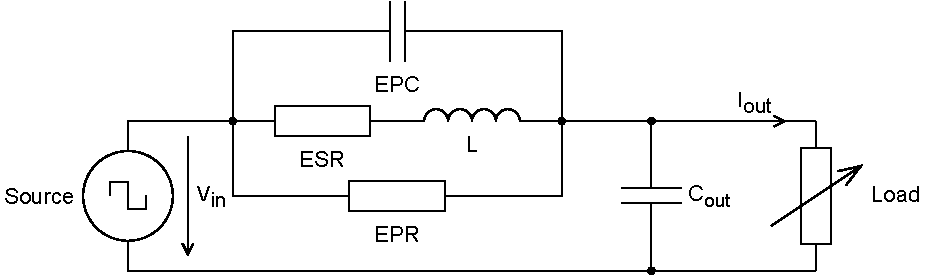
\includegraphics[width=1\linewidth]{Bilder/Kapitel4/Saturation_Validation_ECM.pdf}
    \caption{Circuit Diagram simulating the behaviour of a buck converter}
    \label{fig:saturation_validation_circuit_diagramm}
\end{figure}
The voltage source sends out rectangular voltage pulses with a 50\% duty cycle, \SI{30}{\V} peek at a switching frequency of \SI{300}{\kilo\Hz}. Measuring the peek-to-peek amplitude of the ripple current flowing through the \ac{ECM}, the current drawn by the simulated load is increased step by step from \SI{0.5}{\A} to \SI{20}{\A}. This process is then repeated for all five inductors.\\
Similarly for the physical measurement, the buck converter is set to the same settings and uses the setup described in section \ref{sec:setup_of_the_buck_converter}. Choosing \textit{EPC2308} as the switching element, results in a high efficiency of the buck converter, minimizing the distortion of the measurements. 
\subsection{Comparison of the Simulated and Measured Saturation Behaviour}
Observing the measured data of the physical buck converter, a \ac{DC} dependent increase of the ripple currents amplitude is detected for all inductors. This increase, however, is not uniform between the inductors. For the \textit{SER1512} inductors, their ripple current scales up drastically, as soon as the approximate saturation current of \SI{7}{\A} and \SI{10}{\A} is reached. At \SI{20}{\A} \ac{DC} both register a peek-to-peek ripple current amplitude of more than \SI{15}{\A}. In comparison, the \textit{XGL1313} inductors only increase their ripple current amplitude slightly after reaching saturation. Furthermore, the \textit{UA8014-AL} inductor's ripple current amplitude first increases quickly after reaching saturation but then slows down.
\begin{figure}[H]
    \centering
    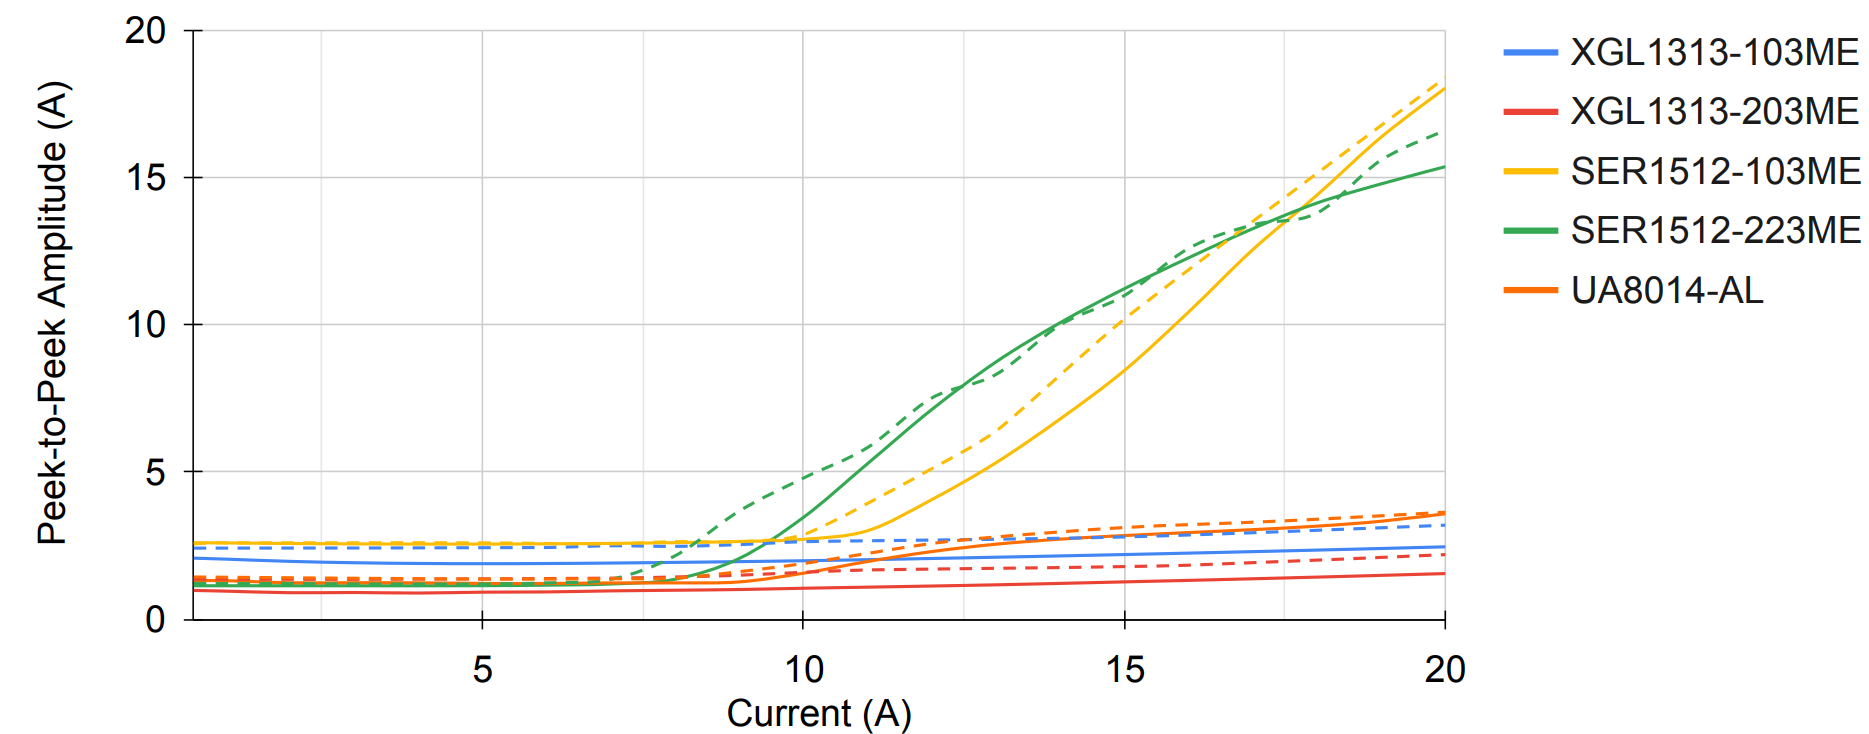
\includegraphics[width=1\linewidth]{Bilder//Kapitel4/High Current_2.png}
    \caption{Ripple current amplitude for high currents \\striped lines indicate measured values, while continuous lines are simulated}
    \label{fig:ripple_current_amplitude_for_high_currents}
\end{figure}
This behaviour mirrors the measured saturation curves. As seen in figure \ref{fig:comparison_of_saturation} the \textit{SER1512} experience a large inductance drop at saturation, while the \textit{XGL1313} gradually decrease their inductance. Due to this, the ripple current amplitude for a high \ac{DC} through the \textit{XGL1313} inductors, does not increase as drastically, as for the \textit{SER1512} inductors. As the \textit{UA8014-AL} contains a plateau in its saturation behaviour, the ripple current amplitude plateaus too after saturation.\\\\
Regarding the simulated peek-to-peek amplitudes, their global behaviour reflects the behaviour of the real inductor well. For the inductors with a sharp inductance drop, their ripple current amplitude in the simulation increases rapidly too, while for the inductors with a gradual inductance decrease, their ripple current amplitude also increases gradually. While discrepancies are present, these are expected due to two main reasons. Firstly measurement errors in the peek-to-peek amplitudes of the physical buck converter introduce noise, most clearly seen for inductor \textit{SER1512-223ME}. Secondly the saturation model is not able to represent the effects of \ac{DC} bias in the physical inductors. But even though this is the case, the saturation model stays valid for both low currents, where saturation is not a factor, as well as high currents, where \ac{DC} bias has it's greatest effect. \\

Having shown, that the saturation model is able to both recreate the saturation behaviour in isolation in section \ref{sec:saturation_behaviour_of_the_inductor} and in combination with the \ac{ECM} under buck converter specific excitation, this model is now implemented into a complete buck converter simulation.

\section{LTspice Simulation of the Buck Converter}\label{sec:complete_simulation_of_the_buck_converter}
Having validated the created inductor model, a complete synchronous buck converter is now created in LTspice, mirroring the physical model created in section \ref{sec:setup_of_the_buck_converter}. 
\subsection{Setup of the Complete Buck Converter Simulation}
Simulating the full synchronous buck converter in LTspice is done by expanding the \ac{ECM} shown in figure \ref{fig:saturation_validation_circuit_diagramm} to include the GaNFET models, provided by EPC. The equivalent inductor model is implemented, consisting of the \ac{ECM} and saturation model introduced in chapter \ref{sec:cha3}.
To convert the given circuit into that of the buck converter, two \acp{GaNFET} models are added in a half-bridge formation. Each \ac{GaNFET} is controlled by a voltage source connected between the \ac{GaNFET}'s source and gate, applying a \SI{6.3}{\V} rectangular signal in accordance with the switching frequency and dead time. 
The different equivalent circuit parameters for the individual inductors are stored in a table and stepped through in each simulation. For the saturation a piecewise function is created containing all saturation functions, which are then selected based on the active inductor model. Enabling the Switching between the different \acp{GaNFET} cannot be realised in the same way, as they are implemented as subnets, necessitating a separate buck converter model for each \ac{GaNFET}. The input voltage source is changed to output a constant \SI{30}{\V}.
\begin{figure}[H]
    \centering
    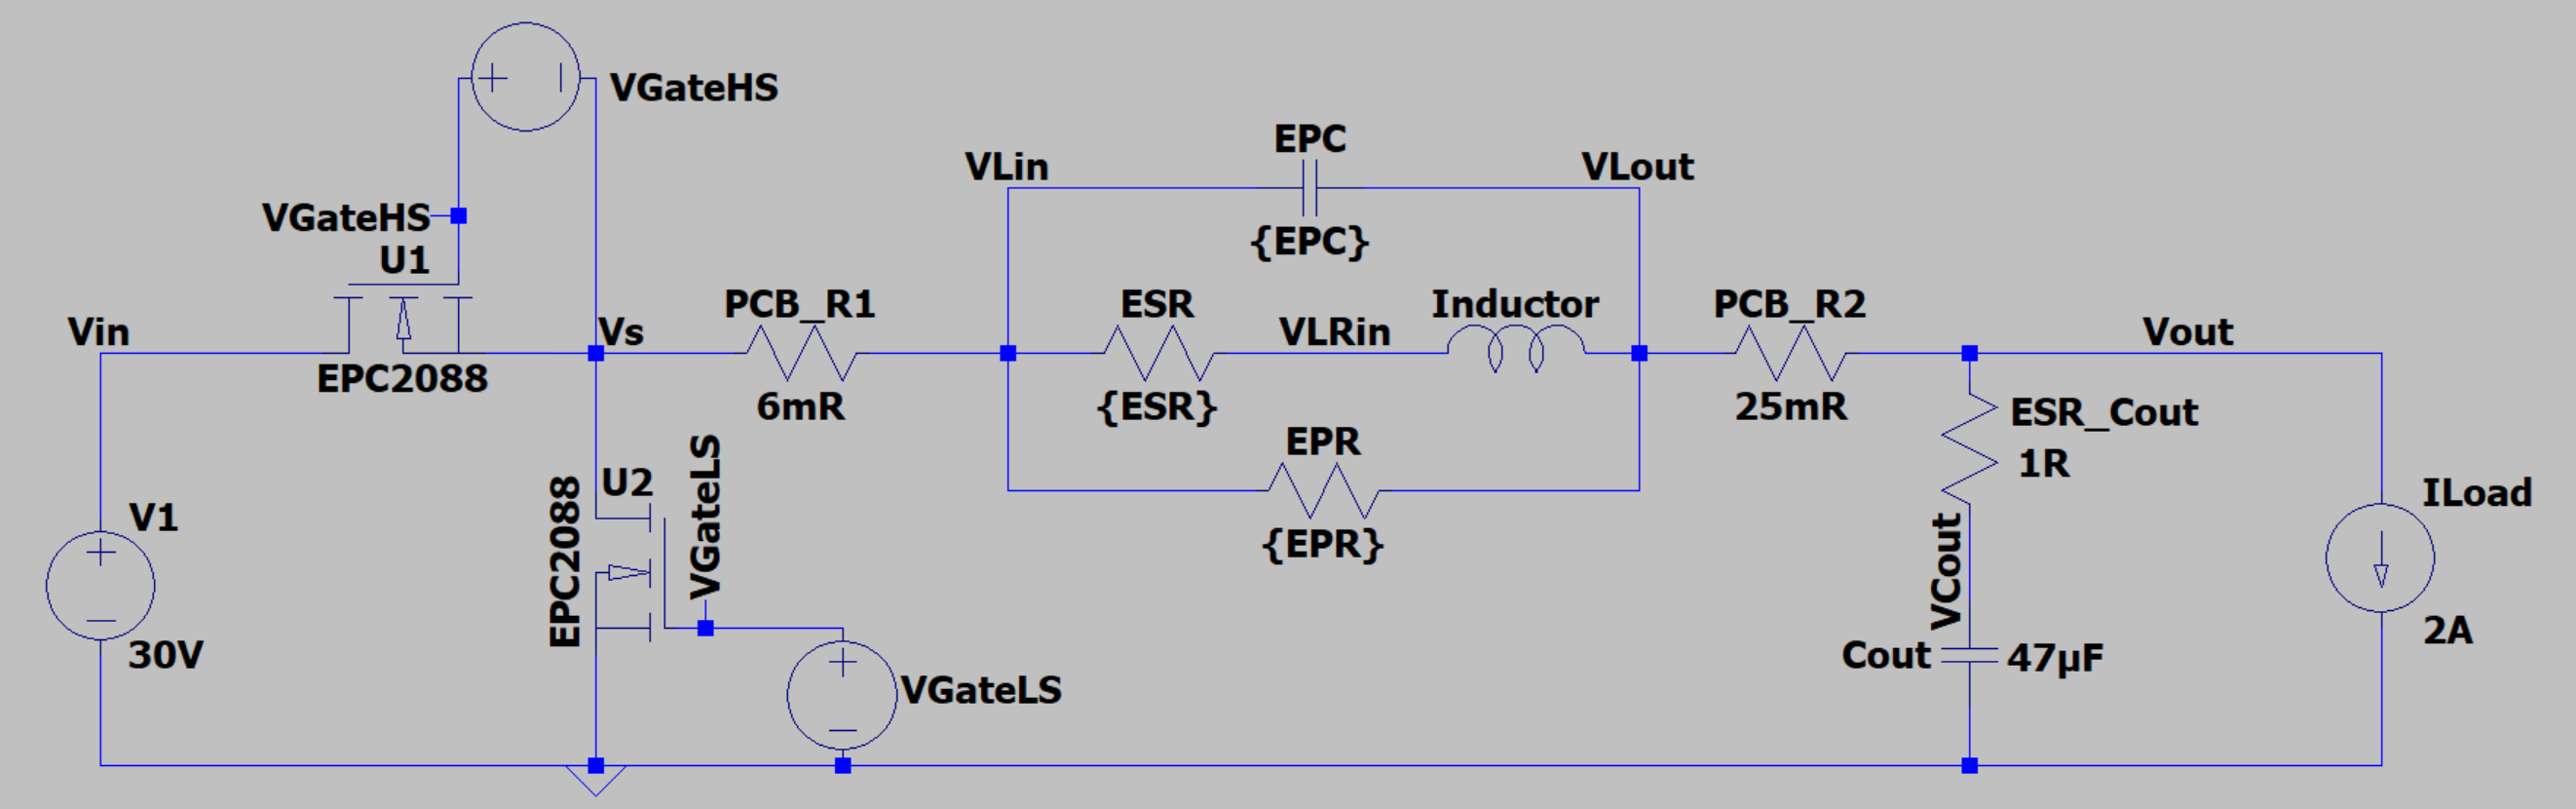
\includegraphics[width=1\linewidth]{Bilder//Kapitel4/BC_LTspice.png}
    \caption{Complete Synchronous Buck Converter in LTspice with the \textit{EPC2088}}
    \label{fig:BC_LTspice}
\end{figure}
Measuring the individual currents, voltages and powers is done via the \textit{.meas}-command, which outputs the average of the observed functions for each given switching frequency and buck converter to an external file. To calculate this average, LTspice simply adds up the values of its output graph, only taking into account the displayed part of the signal. Because of this, it is crucial that always a whole number of periods is displayed, to create an accurate measurement. The buck converter is therefore given a set amount of time to settle after which ten periods are displayed and used for the measurements. 